

\newcommand{\abA}{4.25in}
\newcommand{\abO}{2.00in}
\newcommand{\abT}{2.75in}

\vspace{.10in}
\centerline{\Large \bf Accelerating Data Analysis with Visualization Recommendation}
% \vspace{.05in}
% \centerline{\Large \bf Validating Design Guidelines for Data Visualization}
\vspace{.10in}
\centerline{Kanit Wongsuphasawat and Dominik Moritz}
\vspace{-.1in}
\begin{center}
	{\bf Areas of Interests:} User Interfaces, Visualization, Recommender Systems, Data Analysis
\end{center}

% kanitw: do we need a citation here?
As business and academia become increasingly data-driven,
more and more data “analysts” may be novices in statistics and data visualization.
Accordingly, it becomes important for tools to better guide users towards
productive analytic processes and effectively designed visualizations.

For example, consider an analyst examining Broadband Internet Subscription per Population (\textit{Subscription}) over time in South American countries. As a line chart is a well-suited representation for temporal data, our system will recommend a line chart showing average \textit{Subscription} over \textit{Time} and another line chart showing \textit{Subscription} over \textit{Time} across different \textit{Countries}.  If the analyst becomes interested in the \textit{Subscription} in 2013, our system will subsequently present 2013 data as a sorted bar chart (to facilitate comparison) and also suggest a map (for investigating spatial relationships).  In addition, as \textit{Subscription} is correlated with each country’s \textit{GDP per capita}, our system will recommend a scatterplot to show the relationship between \textit{Subscription} and \textit{GDP per capita}.  With these suggestions (Figure 1), the analyst can quickly examine relationships and generate more hypotheses without having to manually instruct software to plot each chart one-by-one.


\begin{figure}[!htbp]
\centering
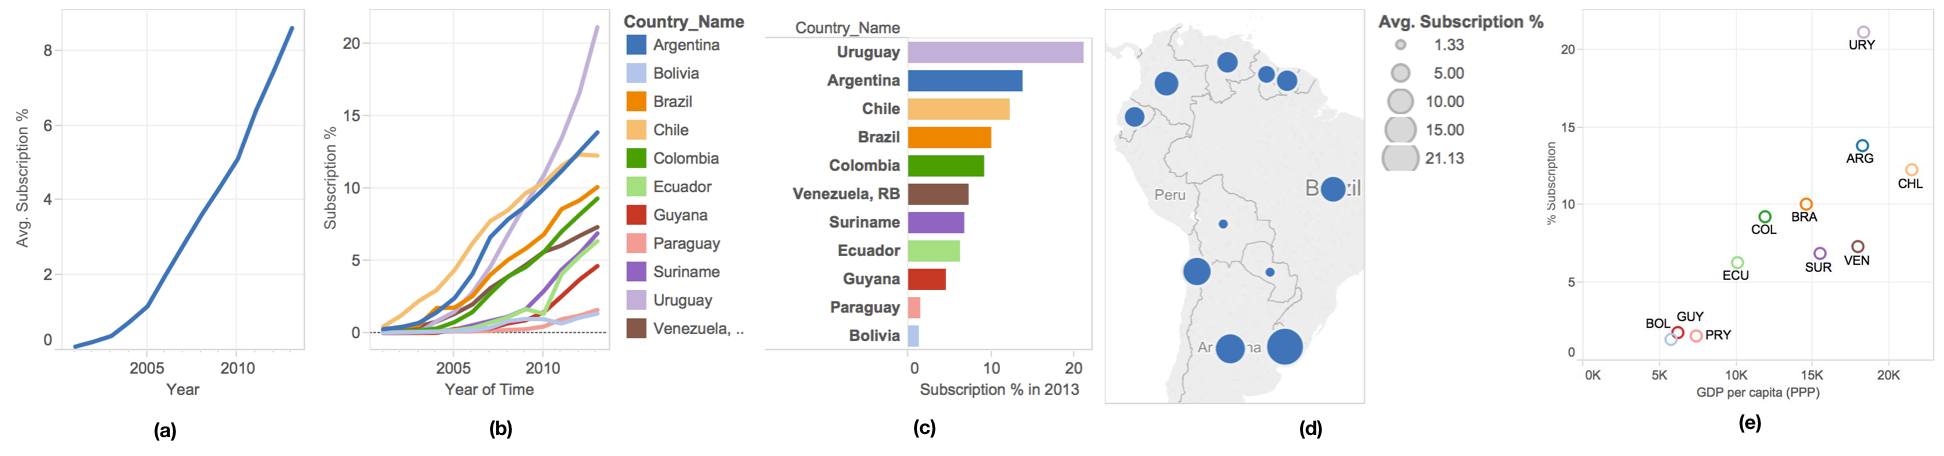
\includegraphics[width=6in]{figure1.png}
\vspace{-0.1in}
\caption{(a,b) line charts showing Broadband Internet Subscription per Population over time in South American countries (on average, and grouped by country respectively) (c,d) a bar chart and a map showing the Subscription in 2013 (e) a scatterplot showing relationship between Subscription and GDP per capita}
\label{fig-examples}
\vspace{-0.15in}
\end{figure}
\vspace{0.1in}

To augment analysts’ ability to perform data analysis, we propose to build a recommender system for visualizing relational data. The system will consist of the following components.

\textbf{1. Interface for Rapid Exploration.}
The interface will include expressive user controls for searching visualizations, enabling analysts to focus on iterative exploration and refinement rather than lower-level design details.

\textbf{2. Comprehensive Recommendation Algorithm.}  What makes a recommendation “good” depends both on the data and task at hand. Accordingly, we will develop a recommendation algorithm that balances user input, best practices (e.g., perceptual effectiveness rankings) for visualization design, data properties and diversity.

\textbf{3. Scalable System.} With larger data, current visualization systems become less responsive or even fail to run at all, preventing rapid exploration.  Furthermore, our recommender system will require expensive querying and modeling operations. We will develop a scalable client-server architecture with the goal of supporting interactive response rates.

